\section{Módulo de Control y Orquestación}
\label{sec:traffic_control}

El módulo \texttt{traffic-control} actúa como orquestador central del sistema distribuido de gestión de tráfico: recibe observaciones vehiculares desde simulaciones o despliegues reales, valida y registra los datos, coordina el envío de información hacia los servicios de optimización (\texttt{traffic-sync}) y almacenamiento distribuido (\texttt{traffic-storage}), y expone una API REST unificada para clientes externos. Su objetivo es desacoplar los productores de datos (por ejemplo, \texttt{traffic-sim}) de los módulos especializados de optimización y persistencia, garantizando un flujo coherente y trazable de información a través del sistema.

% -----------------------------------------------------------------------------
\subsection{Arquitectura del Módulo}
\label{subsec:traffic_control_architecture}

La estructura de \texttt{traffic-control} se organiza en capas bien definidas: configuración, API, modelos de datos, servicios de dominio y utilidades de soporte. El servicio web principal (basado en FastAPI) implementa el punto de entrada \texttt{/process}, que procesa observaciones vehiculares completas, y puntos de entrada auxiliares como \texttt{/healthcheck} y operaciones sobre metadatos. El módulo de configuración centraliza parámetros del sistema, como las URLs de los servicios de almacenamiento y optimización, la cadena de conexión a la base de datos y los niveles de logging. El módulo de configuración de logs define la estructura de registro para toda la aplicación.

La capa de modelos incluye esquemas de validación para estructurar peticiones y respuestas (esquemas de datos, optimización y descarga) y modelos de respuesta estandarizados. El módulo de validación encapsula la validación semántica de los datos: verifica versión de la carga útil, formato de marcas de tiempo, tipo de mensaje (datos u optimización), límites de tamaño de lote (1–10 sensores) e integridad de campos como identificador de semáforo, métricas y estadísticas vehiculares. Cualquier inconsistencia o violación de estos contratos se transforma en una respuesta de error coherente mediante el manejador centralizado de errores.

La persistencia principal del sistema se realiza mediante IPFS y BlockDAG a través del módulo de almacenamiento, que garantiza almacenamiento distribuido, inmutabilidad y trazabilidad verificable. Complementariamente, el módulo de base de datos gestiona un índice auxiliar de metadatos en una base de datos SQL local, con el punto de entrada a la conexión de base de datos y el modelo de metadatos definiendo el esquema de almacenamiento: cada registro guarda, como mínimo, el identificador del semáforo, la marca de tiempo, el tipo de dato (por ejemplo, observación de tráfico u optimización) y referencias a los identificadores de contenido (CIDs y resúmenes criptográficos de transacción) almacenados en el módulo de almacenamiento. El servicio de base de datos proporciona operaciones de alto nivel para crear y consultar este índice local, que se exponen a través de puntos de entrada de metadatos (por ejemplo, \texttt{/metadata/traffic-light/\{id\}}, \texttt{/metadata/recent}, \texttt{/metadata/stats}) para facilitar consultas rápidas, mientras que los datos completos permanecen en el almacenamiento distribuido.

La Figura~\ref{fig:control_architecture} ilustra la arquitectura del módulo \texttt{traffic-control}, mostrando las capas de API, validación, servicios de dominio y persistencia, así como la integración con los módulos especializados del sistema.

\begin{figure}[htbp]
\centering
\shorthandoff{>}
\begin{tikzpicture}[
    node distance=1.0cm,
    api/.style={rectangle, draw, rounded corners, fill=blue!10,
                text width=2.5cm, align=center, minimum height=0.8cm, font=\small},
    service/.style={rectangle, draw, rounded corners, fill=green!10,
                    text width=2.5cm, align=center, minimum height=0.8cm, font=\small},
    storage/.style={rectangle, draw, rounded corners, fill=orange!15,
                    text width=2.8cm, align=center, minimum height=1cm, font=\small},
    db/.style={rectangle, draw, rounded corners, fill=gray!15, dashed,
               text width=1.6cm, align=center, minimum height=0.8cm, font=\tiny},
    arrow/.style={->,thick,>=stealth},
    arrow_aux/.style={->,thick,>=stealth,dashed,gray}
]

    % Cliente
    \node[api] (client) {Cliente\\(traffic-sim)};
    
    % API
    \node[api, below=of client] (api) {API REST\\(FastAPI)};
    
    % Validador
    \node[service, below=of api] (validator) {Validador\\de datos};
    
    % Servicios
    \node[service, below left=1.3cm and 0.5cm of validator] (sync) {Cliente\\traffic-sync};
    \node[service, below right=1.3cm and 0.5cm of validator] (storage) {Cliente\\traffic-storage};
    
    % Almacenamiento distribuido (principal)
    \node[storage, below=2.5cm of storage, xshift=0.5cm] (ipfs) {IPFS + BlockDAG\\(Almacenamiento principal)};
    
    % Base de datos auxiliar
    \node[db, below=2.5cm of validator, xshift=-0.5cm] (db) {\tiny BD SQL\\\tiny Metadatos aux.};
    
    % Flechas principales
    \draw[arrow] (client) -- node[right,font=\scriptsize] {POST /process} (api);
    \draw[arrow] (api) -- (validator);
    \draw[arrow] (validator) -- (sync);
    \draw[arrow] (validator) -- (storage);
    \draw[arrow] (storage) -- node[right,font=\tiny] {Datos} (ipfs);
    
    % Flechas auxiliares (dashed)
    \draw[arrow_aux] (storage) |- node[left,font=\tiny] {CIDs} (db);
    \draw[arrow_aux] (sync) |- node[left,font=\tiny] {Metadatos} (db);

\end{tikzpicture}
\shorthandon{>}
\caption{Arquitectura del módulo \texttt{traffic-control} mostrando el flujo de orquestación. El almacenamiento principal se realiza mediante IPFS y BlockDAG a través de \texttt{traffic-storage}, mientras que la base de datos SQL se utiliza únicamente como índice auxiliar de metadatos.}
\label{fig:control_architecture}
\end{figure}

% -----------------------------------------------------------------------------
\subsection{Flujo de Procesamiento}
\label{subsec:traffic_control_process}

El punto de entrada \texttt{POST /process} es el principal para observaciones de tráfico, tanto provenientes de \texttt{traffic-sim} como de otros clientes. El flujo de procesamiento sigue una secuencia de pasos bien definida:

\begin{enumerate}
    \item \textbf{Recepción y validación}: la API recibe una carga útil en formato unificado (versión 2.0), que puede contener uno o varios sensores asociados a un mismo identificador de semáforo. El módulo de validación verifica que el mensaje cumpla con la estructura esperada (campos obligatorios en métricas y estadísticas vehiculares, rango de tamaño de lote, formatos de fecha, tipo de mensaje), generando errores explícitos en caso de inconsistencias.
    \item \textbf{Preprocesamiento de datos}: el servicio de procesamiento de datos puede aplicar transformaciones ligeras sobre los datos (normalización de campos, ajuste de formatos, enriquecimiento con información temporal) antes de enviarlos a los módulos externos. Esta capa asegura que, aunque distintos productores tengan pequeñas variaciones, el sistema trabaje con un formato interno coherente.
    \item \textbf{Almacenamiento distribuido principal}: el proxy de almacenamiento construye una petición hacia la API del módulo de almacenamiento, que implementa el almacenamiento principal del sistema mediante IPFS y BlockDAG. Los datos completos se almacenan de forma distribuida e inmutable, recibiendo de vuelta identificadores de contenido (CIDs de IPFS) y resúmenes criptográficos de transacción en BlockDAG. Este es el mecanismo de persistencia central del sistema, garantizando trazabilidad, integridad e inmutabilidad de los registros históricos.
    \item \textbf{Índice auxiliar de metadatos}: mediante el servicio de base de datos, se registra en una base de datos SQL local un resumen del evento (identificador de semáforo, marca de tiempo, tipo, estado del procesamiento, CIDs y resúmenes criptográficos de transacción), lo que permite consultas rápidas sobre qué datos fueron recibidos, cuándo y con qué resultado. Esta base de datos actúa únicamente como índice auxiliar para facilitar consultas locales, complementando los registros inmutables almacenados en IPFS y BlockDAG gestionados por el módulo de almacenamiento.
    \item \textbf{Interacción con el módulo de optimización}: el proxy de sincronización envía los datos de tráfico al módulo de optimización mediante el punto de entrada \texttt{/evaluate}, en formato compatible con el sistema difuso y el optimizador PSO. Para lotes de sensores, la función de envío por lotes reempaqueta el lote en el formato esperado por el módulo de optimización (incluyendo el campo de identificador de semáforo de referencia) y recibe un conjunto de optimizaciones, una por grupo detectado.
    \item \textbf{Respuesta al cliente}: finalmente, el servicio de procesamiento compone una respuesta estandarizada utilizando los modelos de respuesta definidos, indicando el estado del procesamiento (por ejemplo, éxito o error), un mensaje descriptivo y, cuando corresponda, datos derivados como tiempos de verde optimizados e impacto estimado sobre la congestión. Esta respuesta se devuelve al cliente original (por ejemplo, el módulo de simulación), que puede aplicar las decisiones de control correspondientes.
\end{enumerate}

Durante todo el flujo, el manejador centralizado de errores proporciona mecanismos para capturar y clasificar errores en distintas categorías (validación, almacenamiento, sincronización, base de datos, errores genéricos), generando respuestas HTTP adecuadas y registros de log con contexto detallado para facilitar la depuración.

% -----------------------------------------------------------------------------
\subsection{Interacción con los Módulos}
\label{subsec:traffic_control_integration}

Desde el punto de vista del sistema global, \texttt{traffic-control} se posiciona como el módulo de orquestación que articula la interacción entre simulación, optimización y almacenamiento distribuido:

\begin{itemize}
    \item \textbf{Relación con \texttt{traffic-sim}}: el módulo de simulación basado en SUMO detecta cuellos de botella y, cuando identifica una situación crítica en una intersección, construye una carga útil con métricas agregadas de tráfico y lo envía a \texttt{traffic-control} mediante el punto de entrada \texttt{/process}. De este modo, \texttt{traffic-sim} no necesita conocer detalles sobre \texttt{traffic-sync} ni \texttt{traffic-storage}; sólo interactúa con un servicio central que gestiona validación, almacenamiento y consulta de optimizaciones.
\end{itemize}

La Figura~\ref{fig:control_sequence} muestra un diagrama de secuencia detallado del flujo completo de procesamiento en \texttt{traffic-control}, ilustrando las interacciones entre todos los componentes del sistema desde la recepción de datos hasta la persistencia distribuida.

\begin{figure}[htbp]
    \centering
    \shorthandoff{>}
    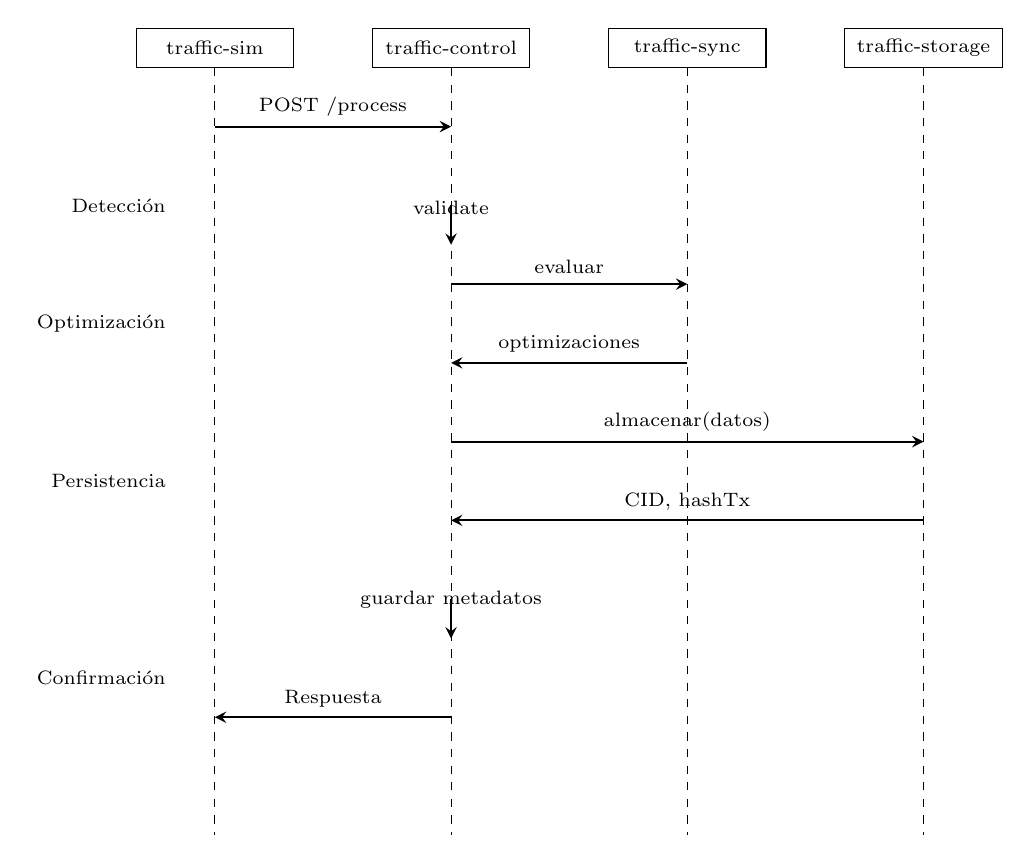
\begin{tikzpicture}[
        >=stealth,
        node distance=0.8cm,
        actor/.style={rectangle, draw, minimum width=2cm, minimum height=0.5cm, font=\scriptsize},
        message/.style={->,thick}
    ]
    
        % Actores
        \node[actor] (sim) at (0,0) {traffic-sim};
        \node[actor] (control) at (3,0) {traffic-control};
        \node[actor] (sync) at (6,0) {traffic-sync};
        \node[actor] (storage) at (9,0) {traffic-storage};
        
        % Líneas de vida
        \draw[dashed] (sim) -- ++(0,-10);
        \draw[dashed] (control) -- ++(0,-10);
        \draw[dashed] (sync) -- ++(0,-10);
        \draw[dashed] (storage) -- ++(0,-10);
        
        % Mensajes
        \draw[message] (0,-1) -- node[above,font=\scriptsize] {POST /process} (3,-1);
        
        \draw[message] (3,-2) -- node[above,font=\scriptsize] {validate} (3,-2.5);
        
        \draw[message] (3,-3) -- node[above,font=\scriptsize] {evaluar} (6,-3);
        \draw[message] (6,-4) -- node[above,font=\scriptsize] {optimizaciones} (3,-4);
        
        \draw[message] (3,-5) -- node[above,font=\scriptsize] {almacenar(datos)} (9,-5);
        \draw[message] (9,-6) -- node[above,font=\scriptsize] {CID, hashTx} (3,-6);
        
        \draw[message] (3,-7) -- node[above,font=\scriptsize] {guardar metadatos} (3,-7.5);
        
        \draw[message] (3,-8.5) -- node[above,font=\scriptsize] {Respuesta} (0,-8.5);
        
        % Etiquetas
        \node[left,font=\scriptsize] at (-0.5,-2) {Detección};
        \node[left,font=\scriptsize] at (-0.5,-3.5) {Optimización};
        \node[left,font=\scriptsize] at (-0.5,-5.5) {Persistencia};
        \node[left,font=\scriptsize] at (-0.5,-8) {Confirmación};
    
    \end{tikzpicture}
    \shorthandon{>}
    \caption{Diagrama de secuencia del flujo completo de procesamiento en el sistema distribuido.}
    \label{fig:control_sequence}
\end{figure}

\begin{itemize}
    \item \textbf{Relación con el módulo de optimización}: \texttt{traffic-control} actúa como cliente del módulo de optimización a través del proxy de sincronización. Para cada observación (o lote) recibida, reenvía los datos relevantes al módulo de optimización, que ejecuta el pipeline de lógica difusa y PSO para producir tiempos de verde optimizados y categorías de congestión. La respuesta del módulo de optimización se integra en la respuesta de \texttt{traffic-control}, permitiendo que los consumidores (por ejemplo, el módulo de simulación) apliquen las configuraciones recomendadas.
    \item \textbf{Relación con el módulo de almacenamiento}: mediante el proxy de almacenamiento, \texttt{traffic-control} sube y recupera datos hacia/desde el módulo de almacenamiento, que a su vez utiliza IPFS, blockchain y BlockDAG como backend de almacenamiento y registro inmutable. \texttt{traffic-control} registra en su base de datos los identificadores de contenido (por ejemplo, CIDs) devueltos por el módulo de almacenamiento, de modo que las consultas de metadatos pueden resolverse localmente y, cuando es necesario, seguir la cadena de referencias hasta los datos almacenados en el sistema distribuido.
\end{itemize}

Esta arquitectura modular permite que cada componente se especialice en su responsabilidad principal: \texttt{traffic-sim} en la generación de escenarios y detección de cuellos de botella; \texttt{traffic-sync} en la evaluación de congestión y optimización de tiempos semafóricos mediante lógica difusa y PSO; \texttt{traffic-storage} en la persistencia verificable de datos; y \texttt{traffic-control} en la validación, coordinación y exposición de un punto de entrada unificado al sistema. En conjunto, estos módulos forman una plataforma escalable y descentralizada para la gestión inteligente de tráfico urbano.

